\clearpage
\item \subquestionpoints{5} \textbf{Coding problem.}
We will now tune the hyperparameter $\tau$.
In \texttt{src/p05c\_tau.py}, find the MSE value of your model on the 
validation set for each of the values of $\tau$ specified in the code. For each
$\tau$, plot your model's predictions on the validation set in the format
described in part (b). Report the value of $\tau$ which achieves the lowest MSE
on the \texttt{valid} split, and finally report the MSE on the \texttt{test}
split using this $\tau$-value.

\ifnum\solutions=1 {
  \begin{answer}

    For $\tau$ = 0.03, MSE on the validation set is: 0.01809616.

    For $\tau$ = 0.05, MSE on the validation set is: 0.01240008.

    For $\tau$ = 0.1, MSE on the validation set is: 0.02422459.

    For $\tau$ = 0.5, MSE on the validation set is: 0.33053127.

    For $\tau$ = 1.0, MSE on the validation set is: 0.40009595.

    For $\tau$ = 10.0, MSE on the validation set is: 0.43374392.

    Best $\tau$ is: 0.05.

    For $\tau$ = 0.05, MSE on the test set is: 0.01699014.

    \begin{figure}[htbp]
        \centering
        \begin{minipage}[t]{0.48\textwidth}
            \centering
            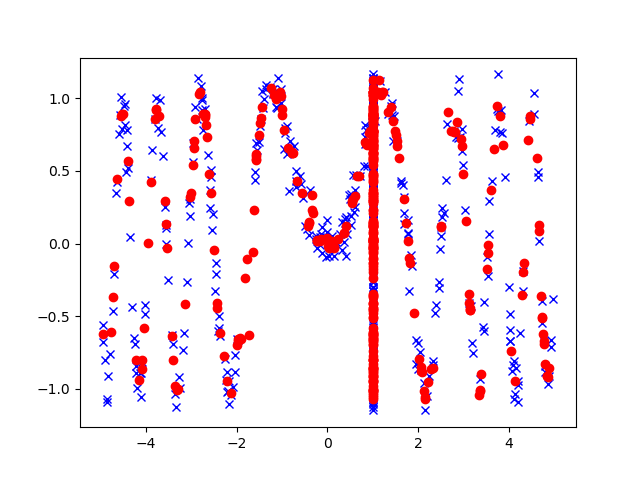
\includegraphics[width=6cm]{../src/output/p05c_1.png}
            \caption{$\tau = 0.03$}
        \end{minipage}
        \begin{minipage}[t]{0.48\textwidth}
            \centering
            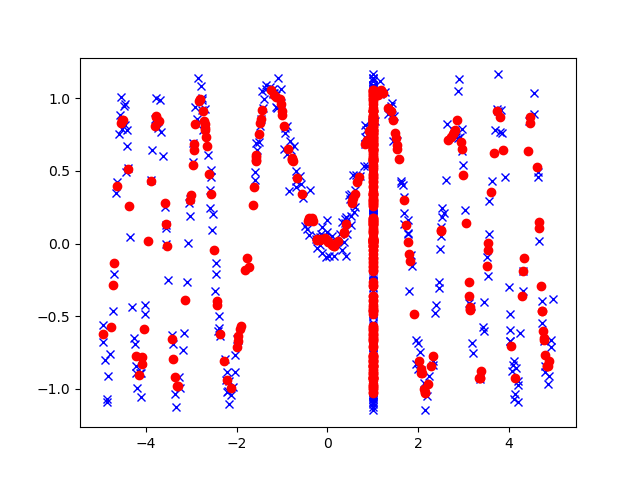
\includegraphics[width=6cm]{../src/output/p05c_2.png}
            \caption{$\tau = 0.05$}
        \end{minipage}
        \begin{minipage}[t]{0.48\textwidth}
            \centering
            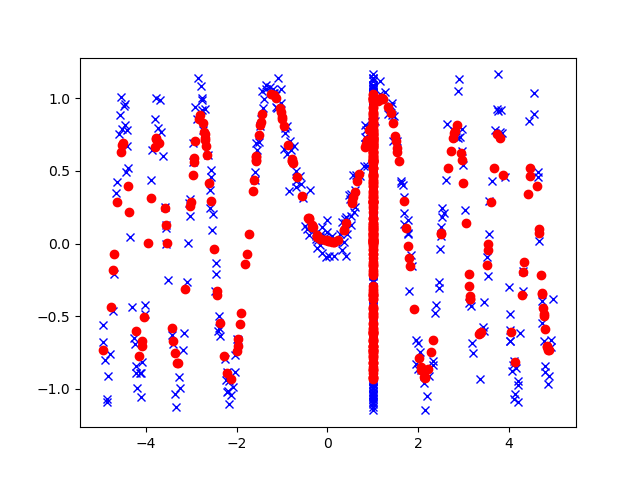
\includegraphics[width=6cm]{../src/output/p05c_3.png}
            \caption{$\tau = 0.1$}
        \end{minipage}
        \begin{minipage}[t]{0.48\textwidth}
            \centering
            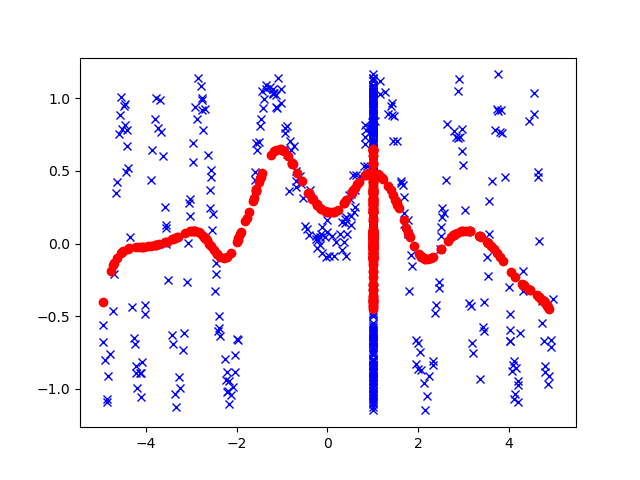
\includegraphics[width=6cm]{../src/output/p05c_4.png}
            \caption{$\tau = 0.5$}
        \end{minipage}
        \begin{minipage}[t]{0.48\textwidth}
            \centering
            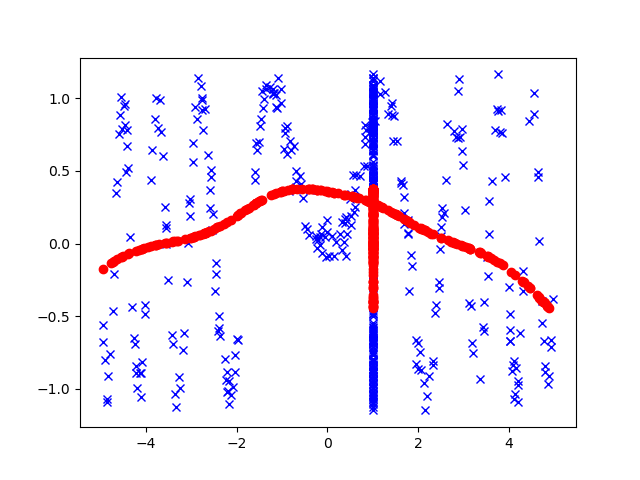
\includegraphics[width=6cm]{../src/output/p05c_5.png}
            \caption{$\tau = 1$}
        \end{minipage}
        \begin{minipage}[t]{0.48\textwidth}
            \centering
            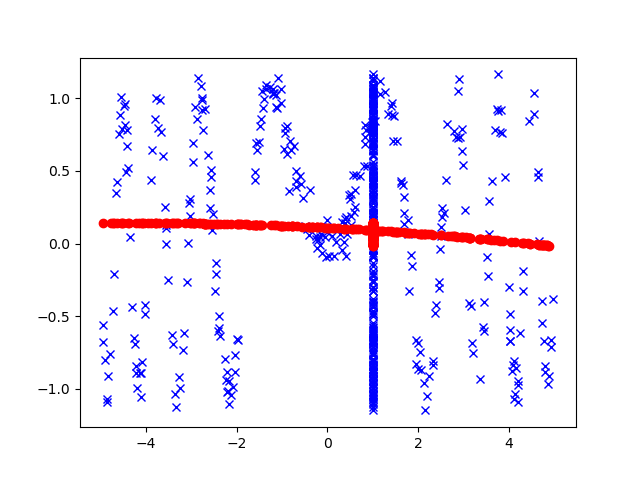
\includegraphics[width=6cm]{../src/output/p05c_6.png}
            \caption{$\tau = 10$}
        \end{minipage}
    \end{figure}
\end{answer}

} \fi
